\documentclass{beamer}
\mode<presentation>
\usepackage{amsmath}
\usepackage{amssymb}
\usepackage{adjustbox}
\usepackage{subcaption}
\usepackage{enumitem}
\usepackage{multicol}
\usepackage{listings}
\usepackage{url}
\usetheme{Madrid}
\usecolortheme{beaver}

\setbeamertemplate{navigation symbols}{}

\numberwithin{equation}{section}

    \title{Assignment 1}
    \author{Tadipatri Uday Kiran Reddy}
    \date{\today} 
    \logo{
\includegraphics[height=1.5cm]{./figs/logo.jpg}}
\begin{document}

\begin{frame}
\titlepage
\end{frame}

\begin{frame}{Question 40}
    For the combined transitional and rotational system shown below, find the transfer function , $G(s) = X(s)/T(s)$.
    \begin{center}
        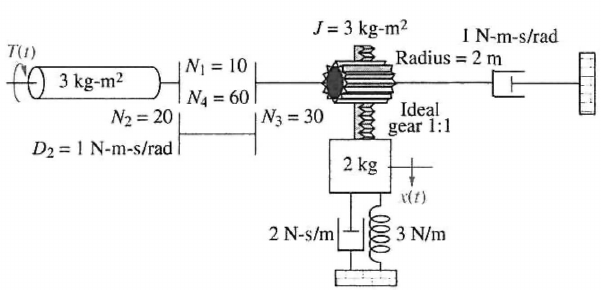
\includegraphics[height= 4cm]{./figs/Question_40.png}
    \end{center}
    
\end{frame}

\begin{frame}{Solution}
     We can solve this problem in two ways,
     \begin{itemize}
         \item --By writing Free body equations.
         \item --Using analogy of electrical mesh equations with mechanical systems.
     \end{itemize}
\end{frame}

\begin{frame}{Analogy of Mesh equations with Mechanical Systems}
    In laplcaian Domain,Free body equations will be,
        \begin{equation*}
            F(s) = M{s^2}{X(s)}; T(s) = J{s^2}{\Theta(s)}\\
            F(s) = K X(s); T(s) = K \Theta(s)\\
            F(s) = f_{v}sX(s); T(s) = f_{v}s\Theta(s)\\
        \end{equation*}
    Since the Mechanical Model is Linear-Time-Invariant Systems, we can add the impedences and in case of\\
    system having N Degrees of Freedom, We can add its Forces also into the final equation,\\
\end{frame}
    
\begin{frame}{Contd.}
     For Eg, A system having 2 DOF,\\
        [Sum of Applied Forces on $X_1$] = $X_1(s)$(Sum of impedences at $X_1$) - $X_2(s)$(Sum of impedences across $X_1$ and $X_2$);\\
        \\[Sum of Applied Forces on $X_2$] = $-X_1(s)$(Sum of impedences across $X_1$ and $X_2$) + $X_2(s)$(Sum of impedences at $X_2$);
\end{frame}

\begin{frame}{Solution}
    One thing we can observe is that there is only one-degree of freedom.\\
    Seeing everything from the Gear's perspective,\\
    All the impedances get scaled up due presence of the gears.\\
    \begin{center}
     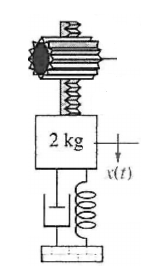
\includegraphics[height = 4cm]{./figs/gear.png}    
    \end{center}
\end{frame}

\begin{frame}{Contd.}
In Laplacian Domain,\\\\
For rotational systems:\\\\
        $T_g = ($Sum of all Impedences about the gear$){\Theta_{g}(s)} + $Torque applied by the transnational motion,\\
Here $T_g$ is torque on gear and $\Theta_g(s)$ is angular displacement of the gear.
    \begin{center}
        \begin{equation*}
            J_e = 3({\frac{N_4N_2}{N_1N_3}}^2) + 3;J_e = 51,\\
            D_e = D_2({\frac{N_2}{N_1}}^2) + 1;D_e = 5,\\
            \implies T_g(s) = (51s^2 + 5s){\Theta_g(s)} + T_{trans}(s) \tag{1} \label{eq:main_eq}
        \end{equation*}
    \end{center}
\end{frame}

\begin{frame}{Contd.}
For transitional systems:\\
$F(s) = (Ms^2 + K + f_vs)X(s)$\\\\
Since, Gear Ratio is 1:1,\\
Torque applied by transnational and rotational is the same,
    \begin{center}
        \begin{equation*}
            \implies T_{on gear}(s) = F(s)r,\\
            r\Theta_g(s) = X(s) \implies \Theta_g = 0.5X(s),\\\\
            \implies T_g(s) = 0.5(51s^2 + 5s)X(s) + r(Ms^2 + K + f_vs)X(s),\\\\
            T_g(s) = \frac{59s^2 + 13s + 12}{2}X(s),\\
        \end{equation*}
    \end{center}
And we know that Torque $\propto$ Number of teeth,\\
$\implies T(s) = (\frac{N_4N_2}{N_1N_3})T_g(s)$.\\
$\implies G(s) = X(s)/T(s) = \frac{X(s)}{4T_g(s)} = \frac{8}{59s^2 + 13s + 12}$\\
\end{frame}

\begin{frame}{Plots}

     \begin{center}
         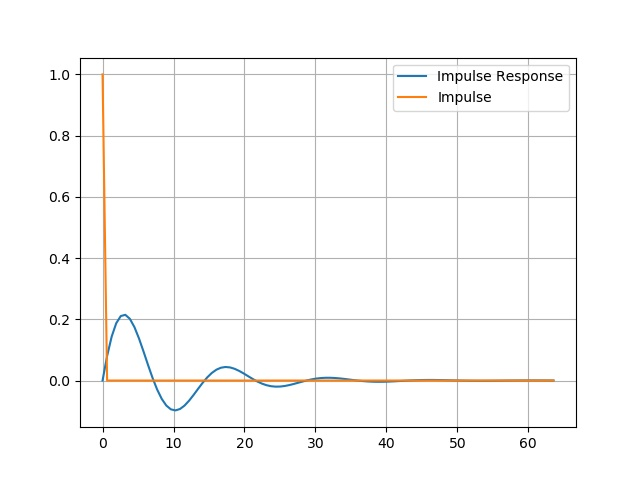
\includegraphics[height = 4cm]{./figs/Impulse Response.jpg}
         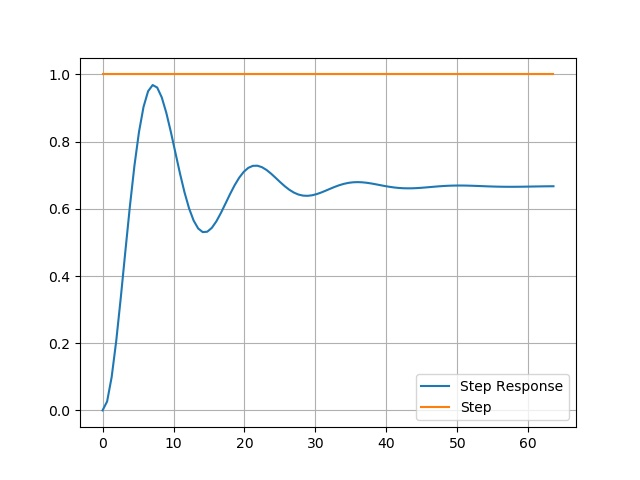
\includegraphics[height = 4cm]{./figs/Step Response.jpg}
     \end{center}
     Find the codes in,\\

        \url{https://github.com/TUdayKiranReddy/Control_Systems/blob/master/Assignment_1/C_2_Q_40.py}

\end{frame}
\end{document}
